\documentclass[../../main.tex]{subfiles}
\begin{document}

\subsection*{7.13}
Una spira rettangolare rigida, di lati $\vec{PQ} = \vec{RS} = a = 20cm$ e $\vec{QR} = \vec{SP} = b = 10cm$, ha una massa per unità di lunghezza $\delta = 5 * 10^{-2} \frac{g}{cm}$ ed è percorsa da una corrente.
\\Essa può ruotare senza attrito intorno a $\vec{PQ}$ che è parallelo all'asse x orizzontale. Quando sulla spira agisce un campo magnetico uniforme e verticale $\vec{B}=B\vec{u_z}$ con $B=2*10^{-2}T$ essa ruota di un angolo $\theta = 30°$.
\\Calcolare il valore della corrente i e il lavoro W fatto dal campo sulla spira durante la rotazione. 
\\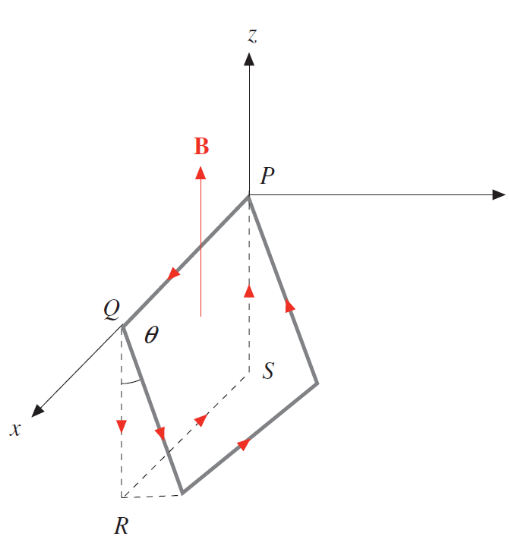
\includegraphics[scale=0.3]{e_7_13.png}
\subsubsection*{Formule utilizzate}
$\vec{m} = i\ S\ \vec{u_n} = i\ a\ b\ \vec{u_n}$
\\$\vec{M} = \vec{m} \wedge  \vec{B} = i\ a\ bB cos\theta\vec{u_x}$
\\$\vec{M_{peso}} = -2\Delta(a+b)\frac{b}{2}gsen\theta\vec{u_x}$
\subsubsection*{Soluzione punto a}
All'equilibrio: $\vec{M} = \vec{M_{peso}}$
\\Andiamo a calcolare la forza peso e il momento sui due bracci posti in $\vec{u_z}$
\\$\vec{M_{PQ}} = \frac{b}{2}sen\theta\Delta b\ g$
\subsubsection*{Soluzione punto b}
da $dW = Md\theta$
\\otteniamo: $W = \int_0^\theta Md\theta$
\\$W = iabB\int_0^{30°}cos\theta d\theta = iabBsin30°$
\\Alternativamente si poteva calcolare come differenza di energia potenziale
\\$W = -(U_p^f - U_p^i) = -U_p^f = i\bigtriangleup \phi(\vec{B})) =iabBcos60° = W$
\newpage

\end{document}